\documentclass{beamer} %

%%%BASICS
\usepackage[utf8]{inputenc}
\usepackage[T1]{fontenc}
\usepackage{lmodern}
\usepackage{amsmath, amssymb}
\usepackage{semantic}
\usepackage{appendix}
\usepackage{babel}
\usepackage{xcolor} % to access the named colour LightGray
\definecolor{LightGray}{gray}{0.9}


\usepackage{pgfplots} % package used to implement the plot

%%%START THEME SETTINGS
\usetheme{CambridgeUS}
\usecolortheme{beaver} % seahorse, dolphin, default, beaver
\usefonttheme{professionalfonts}
\useinnertheme{rectangles}
% \useoutertheme{infolines}

\definecolor{lred}{RGB}{255,245,245}
\definecolor{mred}{RGB}{200,40,40}
\definecolor{dred}{RGB}{170,0,0}

\setbeamercolor{block title}{fg=white,bg=dred}
\setbeamercolor{block body}{bg=lred}
\setbeamercolor{section in toc}{fg=alerted text.fg}
\setbeamercolor{section in toc shaded}{bg=structure!20, fg=mred}
\setbeamercolor{section number projected}{fg=mred, bg=mred,fg=white}
\setbeamercolor{subsection number projected}{fg=mred, bg=mred,fg=white}
\setbeamertemplate{itemize item}{\color{mred}$\blacksquare$}
\setbeamertemplate{itemize item item}{\color{mred}$\blacksquare$}
\setbeamertemplate{enumerate item}{\color{mred}$\bullet$}

\setbeamercovered{transparent}
%%%END THEME SETTINGS

\usepackage{minted}
\usepackage{listings}

\definecolor{codegreen}{rgb}{0,0.6,0}
\definecolor{codegray}{rgb}{0.5,0.5,0.5}
\definecolor{codepurple}{rgb}{0.58,0,0.82}
\definecolor{mgreen}{RGB}{40,150,40}
\definecolor{myellow}{RGB}{244,159,4}
\definecolor{mblue}{RGB}{4,100,244}
\definecolor{mgreen}{RGB}{30,160,8}

\lstdefinestyle{mystyle}{
    backgroundcolor=\color{LightGray},
    commentstyle=\color{mgreen},
    keywordstyle=\color{mred},
    numberstyle=\tiny\color{codegray},
    stringstyle=\color{mgreen},
    basicstyle=\ttfamily\footnotesize,
    breakatwhitespace=false,
    breaklines=true,
    captionpos=b,
    keepspaces=true,
    showspaces=false,
    showstringspaces=false,
    showtabs=false,
    tabsize=2,
}

\lstset{style=mystyle}

\lstdefinelanguage{lustre} {
    morekeywords={node, let, tel, returns, var},
    sensitive=false,
    morecomment=[l]{//},
    morecomment=[s]{/*}{*/},
    morestring=[b]",
    emph={int, unit, float},
    emphstyle=\color{myellow},
    classoffset=1,
    keywords={print, fby},
    keywordstyle=\color{mblue},
    classoffset=0,
}

%------------------------------------------------------
\title[Mini-Lustre $\mapsto$ LLVM]{Compilation de Mini-Lustre vers LLVM}
\institute[UPSaclay]{Université Paris-Saclay}
\author{Lemaire \& Patault}
\date{\today}
%------------------------------------------------------

\newcommand{\ocaml}[1]{\mintinline{ocaml}{#1}}
\newcommand{\llvm}[1]{\mintinline{llvm}{#1}}

\newcommand{\angArr}{
    \rotatebox[origin=c]{180}{$\Lsh$}
}

\pgfplotsset{width=6.5cm, compat=1.17}

\begin{document}
%------------------------------------------------------

\begin{frame}
    \titlepage
\end{frame}

%%%%%%%%%%%%%%%%%%%%%%%%%%%%%%%%%%%%%%%%%%%%%%%%%%%%%%%%%%%%%%%%%%%%%%%%%%%%%%%%%%%%%%%%%%%%%%%%%%%
\section{Introduction}
%%%%%%%%%%%%%%%%%%%%%%%%%%%%%%%%%%%%%%%%%%%%%%%%%%%%%%%%%%%%%%%%%%%%%%%%%%%%%%%%%%%%%%%%%%%%%%%%%%%

\begin{frame}
    \tableofcontents[currentsection]
\end{frame}

\begin{frame}[fragile]{Présentation Générale}
            \vfill
    \begin{itemize}
        \item LLVM := Low Level Virtual Machine

        \vfill\item LLMV IR := langage intermédiare que l'on utilise

        \vfill\item Utilisé par Rust, Clang, \ldots

        \vfill\item Interface C++ et bindings OCaml
    \end{itemize}
            \vfill
\end{frame}

%%%%%%%%%%%%%%%%%%%%%%%%%%%%%%%%%%%%%%%%%%%%%%%%%%%%%%%%%%%%%%%%%%%%%%%%%%%%%%%%%%%%%%%%%%%%%%%%%%%
\subsection{Présentation LLVM}
%%%%%%%%%%%%%%%%%%%%%%%%%%%%%%%%%%%%%%%%%%%%%%%%%%%%%%%%%%%%%%%%%%%%%%%%%%%%%%%%%%%%%%%%%%%%%%%%%%%

\begin{frame}{Pourquoi compiler vers LLVM ?}
    \vfill
    \begin{itemize}
        \item “Assembleur de haut niveau”
        \begin{enumerate}
            \item Typage
            \item Pointeurs
            \item Vecteurs
            \item Tableaux
            \item Structures
            \item Fonctions
            \item ...
        \end{enumerate}
    \vfill \item Bindings simples d'utilisation
    \vfill \item Compilateur optimisant vers toutes les architectures
    \end{itemize}
    \vfill
\end{frame}

%%%%%%%%%%%%%%%%%%%%%%%%%%%%%%%%%%%%%%%%%%%%%%%%%%%%%%%%%%%%%%%%%%%%%%%%%%%%%%%%%%%%%%%%%%%%%%%%%%%
\subsection{Utilisation LLVM}
%%%%%%%%%%%%%%%%%%%%%%%%%%%%%%%%%%%%%%%%%%%%%%%%%%%%%%%%%%%%%%%%%%%%%%%%%%%%%%%%%%%%%%%%%%%%%%%%%%%

\begin{frame}{Schéma de compilation simplifié}
    \begin{overprint}
    \onslide<1>
        \begin{figure}
            \centering
            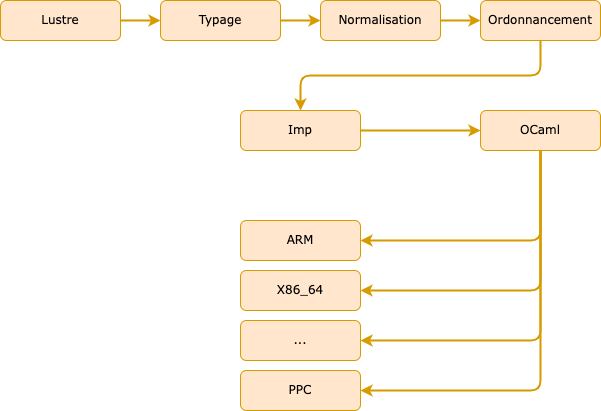
\includegraphics[width=0.8\textwidth]{imgs/compilation0.png}
        \end{figure}
    \onslide<2->
        \begin{figure}
            \centering
            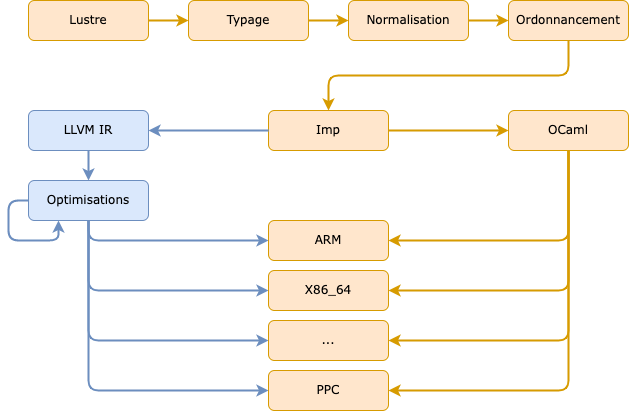
\includegraphics[width=0.82\textwidth]{imgs/compilation1.png}
        \end{figure}
    \end{overprint}

\end{frame}


\begin{frame}[fragile]{En pratique}
    \vfill
    \begin{itemize}
        \item Interface C++ et bindings OCaml
        \begin{minted}
            [baselinestretch=1.1,escapeinside=||,bgcolor=LightGray,fontsize=\footnotesize]
            {ocaml}
    let main = Llvm.declare_function "main" i32_typ in
    let entry_block = (Llvm.basic_blocks func).(0) in
    Llvm.position_at_end entry_block llvm_builder;
    let o = Llvm.build_alloca llvm_typ "o" llvm_builder in
    let one = Llvm.const_int i32_typ 1 in
    let store = Llvm.build_store o one llvm_builder in
    |$\qquad\vdots$|
        \end{minted}
        \vfill\item
        Génération du code LLVM IR (fichiers .ll)
        \begin{minted}
            [baselinestretch=1.1,escapeinside=||,bgcolor=LightGray,fontsize=\footnotesize]
            {llvm}
    declare i32 @main() #0 {
      entry:
        %o = alloca i32, align 4
        store i32 1, i32* %o, align 4
    |$\qquad\vdots$|
        \end{minted}
    \end{itemize}
\vfill
\end{frame}

%%%%%%%%%%%%%%%%%%%%%%%%%%%%%%%%%%%%%%%%%%%%%%%%%%%%%%%%%%%%%%%%%%%%%%%%%%%%%%%%%%%%%%%%%%%%%%%%%%%
\section{Travail Réalisé}
%%%%%%%%%%%%%%%%%%%%%%%%%%%%%%%%%%%%%%%%%%%%%%%%%%%%%%%%%%%%%%%%%%%%%%%%%%%%%%%%%%%%%%%%%%%%%%%%%%%

\begin{frame}
    \tableofcontents[currentsection]
\end{frame}

%%%%%%%%%%%%%%%%%%%%%%%%%%%%%%%%%%%%%%%%%%%%%%%%%%%%%%%%%%%%%%%%%%%%%%%%%%%%%%%%%%%%%%%%%%%%%%%%%%%
\subsection{Dans le dur}
%%%%%%%%%%%%%%%%%%%%%%%%%%%%%%%%%%%%%%%%%%%%%%%%%%%%%%%%%%%%%%%%%%%%%%%%%%%%%%%%%%%%%%%%%%%%%%%%%%%

\begin{frame}[fragile]{Choix de représentation}
    \begin{itemize}
        \item tuple lustre $\to$ structure llvm \\


            \begin{columns}

                \begin{column}{0.1\textwidth}
                \end{column}
                \begin{column}{0.3\textwidth}
%                         \begin{lstlisting}[language=lustre]
% (a:int, b:float) \end{lstlisting}

                    \ocaml{(a:int,b:float)} $\mapsto$
                \end{column}
                \begin{column}{0.6\textwidth}  %%<--- here
                        \begin{minted}[fontsize=\small]{llvm}
%tuple_t_0 = type {i32, float}
                        \end{minted}
                \end{column}
            \end{columns}
    \end{itemize}
\end{frame}

\begin{frame}[fragile]{Exemple de transformation}
    \begin{columns}
    \begin{column}{0.30\textwidth}
        \begin{figure}
        \begin{lstlisting}[language=lustre]
 node f (x:int)
 returns (o:int);
 let
     o = 1;
 tel \end{lstlisting}
            \caption{in.mls}
        \end{figure}

    \end{column}
    \begin{column}{0.05\textwidth}
        $\mapsto$
    \end{column}
    \begin{column}{0.65\textwidth}  %%<--- here
        \begin{figure}
    \begin{minted}[baselinestretch=1.2,bgcolor=LightGray,fontsize=\footnotesize]{llvm}
define i64 @f_1_step(i32 x) {
  %o = alloca i32, align 4
  store i32 1, i32* %o, align 4
  %0 = alloca %ret_f_1_step, align 8
  %1 = getelementptr inbounds ret_f_1_step,
            %ret_f_1_step* %0, i32 0, i32 0
  %2 = load i32, i32* %o, align 4
  store i32 %2, i32* %1, align 4
  %3 = bitcast %ret_f_1_step* %0 to i64*
  %4 = load i64, i64* %3, align 4
  ret i64 %4
}
   \end{minted}
            \vspace{-1cm}
            \caption{out.ll}
        \end{figure}
    \end{column}
    \end{columns}
\end{frame}

%%%%%%%%%%%%%%%%%%%%%%%%%%%%%%%%%%%%%%%%%%%%%%%%%%%%%%%%%%%%%%%%%%%%%%%%%%%%%%%%%%%%%%%%%%%%%%%%%%%
\subsection{Benchmarks}
%%%%%%%%%%%%%%%%%%%%%%%%%%%%%%%%%%%%%%%%%%%%%%%%%%%%%%%%%%%%%%%%%%%%%%%%%%%%%%%%%%%%%%%%%%%%%%%%%%%

\begin{frame}[fragile]{Lustre}
    \begin{figure}
        \begin{lstlisting}[language=lustre]
    node t () returns (i: int);
    let
      i = 1 fby i + 1;
    tel

    node n (u: unit) returns (o: unit);
    var i: int;
    let
      i = t ();
      o = print("coucou", i);
    tel
        \end{lstlisting}
        \caption{Fichier simple.mls}
    \end{figure}

\end{frame}

\begin{frame}{Performances}
    \begin{table}[h]
        \begin{center}
            \begin{tabular}{|r|c|c|}\hline
                                & simple.mls ($10^7$) & simple.mls ($10^8$) \\ \hline\hline
                          LLVM  & 13.84s              & 140.70s             \\ \hline
                          OCaml & 16.29s              & 185.49s             \\ \hline
                          % Lustre compiler & 11s       & 9s        & 19s       \\ \hline
            \end{tabular}
            \caption{Table des performances comparées en fonction du langage cible}
        \end{center}
    \end{table}
\end{frame}

%%%%%%%%%%%%%%%%%%%%%%%%%%%%%%%%%%%%%%%%%%%%%%%%%%%%%%%%%%%%%%%%%%%%%%%%%%%%%%%%%%%%%%%%%%%%%%%%%%%
\subsection{Démonstration}
%%%%%%%%%%%%%%%%%%%%%%%%%%%%%%%%%%%%%%%%%%%%%%%%%%%%%%%%%%%%%%%%%%%%%%%%%%%%%%%%%%%%%%%%%%%%%%%%%%%

\begin{frame}{Démonstration}
    \centerline{C'est parti}
\end{frame}


\end{document}
